% !TEX TS-program = pdflatex
% !TEX encoding = UTF-8 Unicode

% Copyright (c) 2011, Edd Barrett <vext01@gmail.com>
% 
% Permission to use, copy, modify, and/or distribute this software for any
% purpose with or without fee is hereby granted, provided that the above
% copyright notice and this permission notice appear in all copies.
% 
% THE SOFTWARE IS PROVIDED "AS IS" AND THE AUTHOR DISCLAIMS ALL WARRANTIES
% WITH REGARD TO THIS SOFTWARE INCLUDING ALL IMPLIED WARRANTIES OF
% MERCHANTABILITY AND FITNESS. IN NO EVENT SHALL THE AUTHOR BE LIABLE FOR
% ANY SPECIAL, DIRECT, INDIRECT, OR CONSEQUENTIAL DAMAGES OR ANY DAMAGES
% WHATSOEVER RESULTING FROM LOSS OF USE, DATA OR PROFITS, WHETHER IN AN
% ACTION OF CONTRACT, NEGLIGENCE OR OTHER TORTIOUS ACTION, ARISING OUT OF
% OR IN CONNECTION WITH THE USE OR PERFORMANCE OF THIS SOFTWARE.

\documentclass{beamer}

\usetheme{AnnArbor}
\usecolortheme{crane}
\usepackage{helvet}
\usepackage{listings}

\title{Reversing a Simple Shellcode with Radare2}
\subtitle{
\includegraphics[width=.25\textwidth]{r2.png}}
\author{Edd Barrett}
\date{\today}
\institute{@vext01}

\lstset{
  basicstyle=\ttfamily\small,
  breaklines=true,
  stringstyle=\ttfamily,
  frame=tlbr,
  framexleftmargin=1pt,
  backgroundcolor=\color{white}
}


%\AtBeginSection[]{%
%\begin{frame}
%\partpage
%\tableofcontents[currentsection]
%\end{frame}
%}

\begin{document}

\begin{frame}
  \titlepage
  \vspace{-4em}
  \begin{center}
  
\includegraphics[width=.25\textwidth]{qr.png}\\
  Twitter: @radareorg\hfill www: http://radare.org
  \end{center}
\end{frame}

\section{Introducing Radare2}

\begin{frame}[fragile]
\frametitle{\insertsection}

\begin{block}{What is Radare2?}
Radare2 is an open-source framework to aid reversing and modification of binary files.
\end{block}

\vfill

\begin{block}{Some features}
\begin{itemize}
\item Multi-architecture and multi-platform
\item Hex editor
\item Debugger
\item Disassembler
\item \ldots
\end{itemize}
\end{block}

\vfill

\begin{block}{Developers}
@trufae, @nibble\_ds, @earada and handful of testers and contributors.
\end{block}

\end{frame}

\section{Shellcodes}
\begin{frame}
  \frametitle{\insertsection}

  \begin{block}{Definition}
  "Shellcode" is a term colloquially used to refer to the payload of an
  exploit. Typically this would be code injected to start a shell.    
  \end{block}

  \vfill

  \begin{itemize}
    \item Not to be confused with ``Shell Script''.
    \vfill
    \item See \url{http://www.projectshellcode.com/} for examples.
  \end{itemize}
\end{frame}

\section{An Example -- What does this code do?}
\begin{frame}
  \frametitle{\insertsection}

  \lstinputlisting{small-code.c}

  \footnote{Thanks to ``Gunslinger'' for this example}

\end{frame}

\section{Overlapping Registers in x86/x64}

\begin{frame}
  \frametitle{\insertsection}

  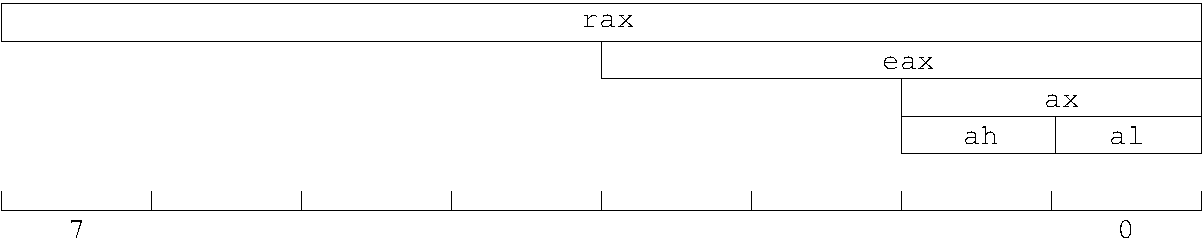
\includegraphics[width=\textwidth]{rax}
  \vfill

\begin{block}{Register Configuration due to Legacy}
  \begin{itemize}
    \item In the 16-bit days we had \texttt{ax}
      \begin{itemize}
        \item High and low byte addressable via \texttt{ah}, \texttt{al}
      \end{itemize}
    \item In the 32-bit days we also had \texttt{eax}
    \item The newest x64 register has \texttt{rax}
  \end{itemize}
\end{block}

\begin{center}
Similarly for \texttt{bx, cx, dx}.
\end{center}

\end{frame}



\section{CALL}
\begin{frame}
  \frametitle{\insertsection}

  \begin{block}{From the Intel Manual}
    Saves procedure linking information on the stack and branches to the called
procedure specified using the target operand.
  \end{block}

  \vfill

  \begin{center}
  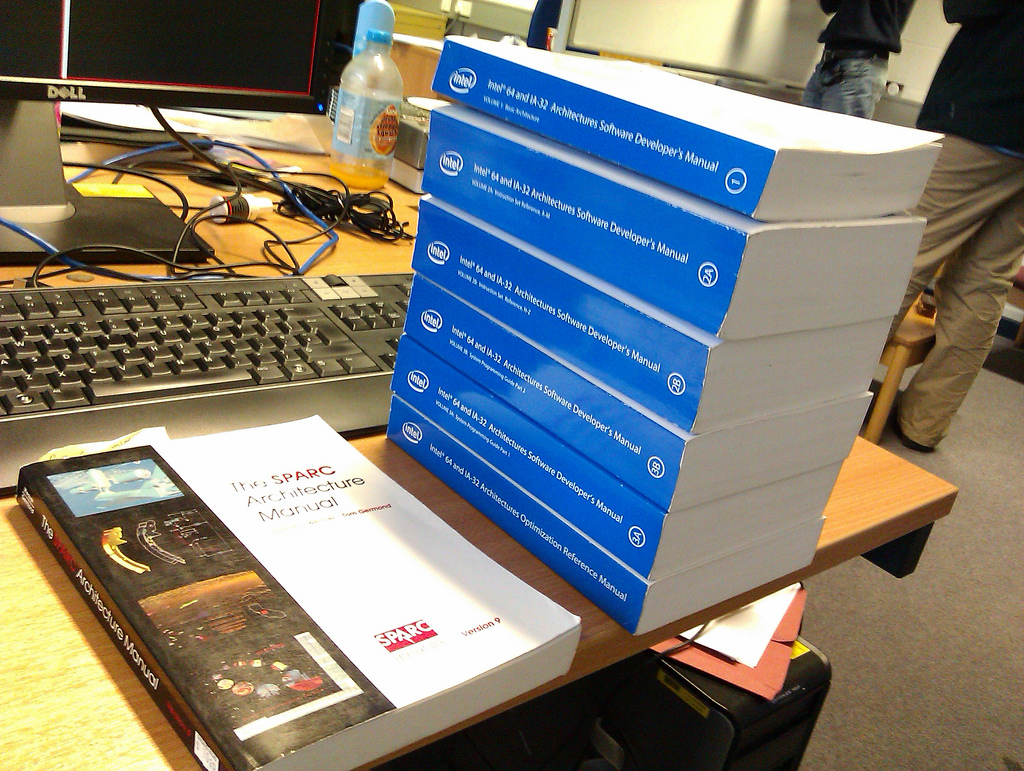
\includegraphics[width=.5\textwidth]{manual.jpg}
  \end{center}

\end{frame}


\section{CALL Example}
\begin{frame}[fragile]
  \frametitle{\insertsection}

\begin{lstlisting}[basicstyle=\footnotesize\tt]
0x1c000286   16    e8e1ffffff       call dword 0x1c00026c
0x1c00028b   16    81               ...
\end{lstlisting}

\vfill

\begin{tabular}{ccc}
Before CALL&&After CALL\\
\\
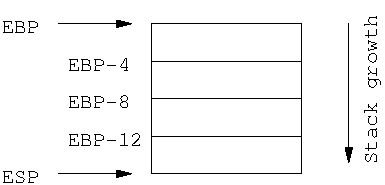
\includegraphics[width=.44\textwidth]{stack1.pdf}&
~~~~~~~\pause&
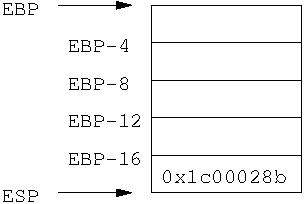
\includegraphics[width=.37\textwidth]{stack2.pdf}\\
\end{tabular}
\end{frame}


\section{System Calls}
\begin{frame}[fragile]
  \frametitle{\insertsection}

\begin{block}{Definition}
The userland can request services from the kernel by calling special functions
known as ``system calls''.
\end{block}

\begin{block}{How do they work?}
\begin{itemize}
\item System calls are not called with the \texttt{CALL} instr\\
\vfill
\item Instead an 0x80 interrupt is fired\\
  \begin{itemize}
  \item The system call number to execute is in \texttt{eax}\\
  \item Arguments should be in $\{$ \texttt{ebx, ecx, edx, esi, edi, ebp}$\}$\\
  \end{itemize}
\end{itemize}
\end{block}

\end{frame}

\section{This Exploit Worked Once...}
\begin{frame}[fragile]
  \frametitle{\insertsection}

\begin{block}{Actually\ldots}
\begin{itemize}
  \item The exploit I have just showed you does not work on modern UNIX/Linux ;)\\
  \item NX bit or $W\char`\^X$ prevents such attacks\\
  \item Pages in \texttt{.data} are writable, therefore not also executable.
  \end{itemize}
\end{block}

\end{frame}

\section{Concluding Comments}
\begin{frame}[fragile]
  \frametitle{\insertsection}

\begin{block}{Thanks for Listening}
  \begin{itemize}
  \item Original blog post:
\url{http://canthack.org/2011/07/adventures-with-radare-1-a-simple-shellcode-analysis/}\\
  \item Follow radare2 on twitter: @radareorg\\
  \item Find radare2 on the web: \url{http://radare.org}\
  \item Source code for these slides: \url{https://github.com/vext01/r2-adventures1-talk}
  \end{itemize}
\end{block}

\end{frame}

\end{document}
